\section{The Cross Product}\label{sec:cross_product}

``Orthogonality'' is immensely important. A quick scan of your current environment will undoubtedly reveal numerous surfaces and edges that are perpendicular to each other (including the edges of this page). The dot product provides a quick test for orthogonality:  vectors $\vec u$ and $\vec v$ are perpendicular if, and only if, $\dotp uv=0$. 

Given two non--parallel, nonzero vectors $\vec u$ and $\vec v$ in space, it is very useful to find a vector $\vec w$ that is perpendicular to both $\vec u$ and $\vec v$. There is a operation, called the \textbf{cross product}, that creates such a vector. This section defines the cross product, then explores its properties and applications.

\definition{def:cross_product}{Cross Product}
{Let $\vec u =\la u_1,u_2,u_3\ra$ and $\vec v = \la v_1,v_2,v_3\ra$ be vectors in $\mathbb{R}^3$. The \textbf{cross product of $\vec u$ and $\vec v$}, denoted $\crossp uv$, is the vector
\index{vectors!cross product}\index{cross product!definition}
\[
\crossp uv = \la u_2v_3-u_3v_2,u_3v_1-u_1v_3,u_1v_2-u_2v_1\ra.
\]
}

\mnote{.6}{The definition of the cross product may look strange (and complicated) at first, but it's more or less forced by the requirement that it be orthogonal to both $\vec u$ and $\vec v$. To begin to see why, suppose $\vec w = \la a,b,c\ra$ is an arbitrary vector such that $\dotp wu=0$ and $\dotp wv=0$. This gives us the pair of equations
\begin{align*}
u_1a+u_2b+u_3c&=0\\
v_1a+v_2b+v_3c&=0.
\end{align*}
This is a \textit{system of linear equations} in the variables $a$, $b$, and $c$. We'll learn the techniques for solving any such system in Chapter \ref{chapter:linear}, at which point we'll be able to see that (up to a scalar multiple) the solution is given by Definition \ref{def:cross_product}.}

This definition can be a bit cumbersome to remember. After an example we will give a convenient method for computing the cross product. For now, careful examination of the products and differences given in the definition should reveal a pattern that is not too difficult to remember. (For instance, in the first component only 2 and 3 appear as subscripts; in the second component, only 1 and 3 appear as subscripts. Further study reveals the order in which they appear.)

Let's practice using this definition by computing a cross product.\\

\example{ex_crossp1}{Computing a cross product}{
Let $\vec u = \la 2,-1,4\ra$ and $\vec v = \la 3,2,5\ra$. Find $\crossp uv$, and verify that it is orthogonal to both $\vec u$ and $\vec v$.
}
{Using Definition \ref{def:cross_product}, we have
\begin{align*}
\crossp uv &= \la u_2v_3-u_3v_2,u_3v_1-u_1v_3,u_1v_2-u_2v_1\ra\\
		   &= \la (-1)5-(4)2,(4)3-(2)5, (2)2-(-1)3\ra = \la -13,2,7\ra.
\end{align*}
(We encourage the reader to compute this product on their own, then verify their result.)

We test whether or not $\crossp uv$ is orthogonal to $\vec u$ and $\vec v$ using the dot product:
\begin{align*}
\big(\crossp uv\big) \cdot \vec u &= \la -13,2,7\ra \cdot \la 2,-1,4\ra = 0,\\
\big(\crossp uv\big) \cdot \vec v &= \la -13,2,7\ra \cdot \la 3,2,5 \ra = 0.
\end{align*}
Since both dot products are zero, $\crossp uv$ is indeed orthogonal to both $\vec u$ and $\vec v$.
}\\

We now introduce a method for computing the cross-product that is easier to remember, and has the added benefit of allowing us to preview \sword{determinants}, which we will return to in earnest in Section \ref{sec:determinant_1}. 

Consider a rectangular array $\bbm a&b\\c&d\ebm$ of four real numbers $a,b,c$, and $d$. A $2\times 2$ determinant takes any such array and assigns the number $ad-bc$. This is commonly denoted as follows:
\[
\bvm a&b\\c&d\evm = ad-bc.
\]
Most people find it easiest to remember this in terms of the two \textit{diagonals} of the array: we take the product of the two numbers on the \textit{main diagonal} (top-left to bottom-right), and subtract the product of the two numbers on the other diagonal:
\btz [baseline=-3pt,>=stealth]
\node at (0,0) {$\bvm a & b\\ c& d\evm$};
\draw[->,  thin] (-.5,.4) -- (.6,-.6) node[below right] {$ac\vphantom{bd}$};
\draw[->, thin] (0.4,.4) -- (-.6,-.6) node[below left ] {$bd$};
\etz

For example, we have $\bvm 4&-2\\6&3\evm = 4(3)-(-2)(6)=24$. Once we get comfortable with $2\times 2$ determinants, we can write the cross product in terms of them, as follows:
\begin{align}
\crossp uv &= \bvm u_2&u_3\\v_2&v_3\evm \veci - \bvm u_1&u_3\\v_1&v_3\evm\vecj + \bvm u_1&u_2\\v_1&v_2\evm\veck\label{eq:crossdet}\\ 
& = (u_2v_3-u_3v_2)\veci-(u_3v_1-u_1v_3)\vecj + (u_1v_2-u_2v_1)\veck,\nonumber
\end{align}
as before. Now, this might not seem like much of an improvement over the previous formula, so we take things one step further. First, we form a $3\times 3$ array as shown below. 
\[
\bvm \veci&\vecj&\veck\\u_1&u_2&u_3\\v_1&v_2&v_3\evm.
\]
The first row comprises the standard unit vectors $\vec i$, $\vec j$, and $\vec k$. The second and third rows are the vectors $\vec u$ and $\vec v$, respectively. Next, we \textit{expand} our $3\times 3$ array as a vector, where the coefficient of each standard unit vector is given by the $2\times 2$ determinant that's left over when we delete the row and column containing that unit vector. 

For example, if we use $\vec u$ and $\vec v$ from Example \ref{ex_crossp1}, we obtain the array
\[
\bvm \veci&\vecj&\veck \\  2&-1&4\\3&2&5\evm.
\]
The expansion process used to obtain the coefficients of $\veci, \vecj \veck$ looks like the following:

\btz [baseline=-3pt,>=stealth]
\node at (0,0) {$\bvm \fbox{\veci}&\vecj&\veck \\  2&-1&4\\3&2&5\evm\longrightarrow \bvm -1&4\\2&5\evm\veci = -13\veci$};
\draw[thin] (-2.3,.6) -- (-2.3, -.6);
\draw[thin] (-2.5,.4) -- (-.8,.4);
\etz

\btz [baseline=-3pt,>=stealth]
\node at (0,0) {$\bvm \veci&\fbox{\vecj}&\veck \\  2&-1&4\\3&2&5\evm\longrightarrow \bvm 2&4\\3&5\evm\vecj = -2\vecj$};
\draw[thin] (-1.45,.6) -- (-1.45, -.6);
\draw[thin] (-2.3,.4) -- (-.6,.4);
\etz

\btz [baseline=-3pt,>=stealth]
\node at (0,0) {$\bvm \veci&\vecj&\fbox{\veck} \\  2&-1&4\\3&2&5\evm\longrightarrow \bvm 2&-1\\3&2\evm\veck = 7\veck$};
\draw[thin] (-0.85,.6) -- (-0.85, -.6);
\draw[thin] (-2.3,.4) -- (-.6,.4);
\etz

There is one more important detail to note: notice in Equation \eqref{eq:crossdet} that there is a \textbf{minus sign} in front of the coefficient of the unit vector $\vecj$. We need to make sure that the signs in front of each $2\times 2$ determinant follow this $+,\,-,\,+$ pattern when we expand our array as a vector. For the vectors $\vec u$ and $\vec v$ in Example \ref{ex_crossp1}, we end up with the following:
\begin{align*}
\crossp uv & = \bvm \veci&\vecj&\veck \\  2&-1&4\\3&2&5\evm  = \bvm -1&4\\2&5\evm\veci - \bvm 2&4\\3&5\evm\vecj + \bvm 2&-1\\3&2\evm\veck\\
& = -13\veci - (-2)\vecj + 7\veck = \la -13, 2, 7\ra,
\end{align*}
as before. The method will become more clear with a bit of practice.\\

\mnote{.75}{\textbf{Note:} If the minus sign in front of the $\vecj$ coefficient seems out of place to you, it might help to imagine wrapping our $3\times 3$ array around a cylinder (like the label on a tin can). If we read from left to right, \textit{beginning in the $\vecj$ column}, then we should place the $\veck$ column first, followed by the $\veci$ column. For the vectors $\vec{u}$ and $\vec{v}$ in Example \ref{ex_crossp1}, this would result in the coefficient $\bvm 4&2\\5&2\evm = 2$ for the $\vecj$ component, which has the correct sign. However, since our habit is to read starting from the far left, we tend to write the $\veci$ column first, and then introduce the minus sign to compensate.}


\example{ex_crossp2}{Computing a cross product}{
Let $\vecu=\la 1,3,6\ra$ and $\vec v = \la -1,2,1\ra$. Compute both $\crossp uv$ and $\crossp vu$.}
{To compute $\crossp uv$, we form our $3\times 3$ array as prescribed above, and expand it into a vector:
\begin{align*}
\crossp uv &= \bvm \veci & \vecj & \veck\\ 1& 3& 6\\ -1& 2& 1\evm = \bvm 3& 6\\2 &1\evm \veci - \bvm 1 & 6\\ -1& 1\evm\vecj +\bvm 1& 3\\ -1 & 2\evm\veck\\
		& = (3(1)-6(2))\veci -(1(1)-6(-1))\vecj + (1(2)-3(-1))\veck\\
		& = -9\veci-7\vecj+5\veck = \la -9, -7, 5\ra.
\end{align*}
To compute $\crossp vu$, we switch the second and third rows of the above matrix, then expand as before:
\begin{align*}
\crossp vu & = \bvm \veci & \vecj& \veck\\ -1 & 2& 1\\ 1& 3& 6\evm = \bvm 2 &1\\3 &6\evm\veci - \bvm -1& 1\\ 1& 6\evm\vecj + \bvm -1& 2\\ 1 &3\evm\veck\\
		   & = (2(6)-1(3))\veci-((-1)(6)-1(1))\vecj + ((-1)(3)-2(1))\veck\\
		   & = 9\veci+7\vecj -5\veck = \la 9, 7, -5\ra = -\crossp uv.
\end{align*}
Note how with the rows being switched, the products that once appeared on the right now appear on the left, and vice--versa, so that the result is the opposite of $\crossp uv$. We leave it to the reader to verify that each of these vectors is orthogonal to $\vec u$ and $\vec v$.
}\\

\noindent\textbf{\large Properties of the Cross Product}\\

It is not coincidence that $\crossp vu = -(\crossp uv)$ in the preceding example; one can show using Definition \ref{def:cross_product} that this will always be the case. The following theorem states several useful properties of the cross product, each of which can be verified by referring to the definition.

\setboxwidth{15pt}
%\noindent\hskip-50pt\begin{minipage}{\linewidth}
\theorem{thm:cross_prod_prop}{Properties of the Cross Product}
{Let $\vecu$, $\vecv$ and $\vecw$ be vectors in $\mathbb{R}^3$ and let $c$ be a scalar. The following identities hold:
\index{vectors!cross product}\index{cross product!properties}
\begin{enumerate}
	\item \parbox{167pt}{$\crossp uv = -(\crossp vu)$} Anticommutative Property
	\item	\begin{enumerate}
		\item \parbox{145pt}{$(\vec u+\vec v)\times \vecw = \crossp uw+\crossp vw$} Distributive Properties
		\item	$\vec u \times (\vec v+\vec w) = \crossp uv+\crossp uw$
	\end{enumerate}
	\item		$c(\crossp uv) = (c\vecu) \times \vec v = \vecu \times (c\vecv)$
	\item		\begin{enumerate}
		\item \parbox{145pt}{$(\crossp uv)\cdot \vecu = 0$} Orthogonality Properties
		\item	$(\crossp uv)\cdot \vecv = 0$
	\end{enumerate}
	\item		$\crossp uu = \vec 0$
	\item		$\crossp u0 = \vec 0$
	\item		\parbox{167pt}{$\vecu \boldsymbol{\cdot} (\vecv\times\vecw) = (\crossp uv)\boldsymbol{\cdot} \vecw$} Scalar Triple Product
\end{enumerate}
}
%\end{minipage}
\restoreboxwidth

We introduced the cross product as a way to find a vector orthogonal to two given vectors, but we did not give a proof that the construction given in Definition \ref{def:cross_product} satisfies this property. Theorem \ref{thm:cross_prod_prop} asserts this property holds; we leave it as a problem in the Exercise section to verify this.

The algebraic properties of the cross product in Theorem \ref{thm:cross_prod_prop} also give us an additional method for computing the cross product in terms of the unit vectors $\veci, \vecj, \veck$. We know from Property 5 that
\[
\veci\times\veci = \vec 0, \vecj\times\vecj = \vec 0, \veck\times\veck = \vec 0,
\]
and it's easy to check that
\[
\veci\times\vecj = \veck, \vecj\times\veck = \veci, \veck\times\veci=\vecj,
\]
and then Property 1 guarantees that
\[
\vecj\times \veci = -\veck, \veck\times\vecj = -\veci, \veci\times\veck = -\vecj.
\]
Using Properties 2 and 3, we can then compute, for example,
\begin{align*}
\la 2,0,3\ra\times \la -1,4,2\ra & = (2\veci +3\veck)\times (-\veci +4\vecj +2\veck)\\
& = -2(\veci \times \veci)+8(\veci \times\vecj)+4(\veci \times\veck)\\
& \quad \quad-3(\veck\times\veci)+12(\veck\times\vecj)+6(\veck\times\veck)\\
& = \vec 0+8\veck -4\vecj -3\vecj -12\veci + \vec 0 = \la -12, -7, 8\ra.
\end{align*}

Property 5 from the theorem is also left to the reader to prove in the Exercise section, but it reveals something more interesting than ``the cross product of a vector with itself is $\vec 0$.'' Let $\vec u$ and $\vec v$ be parallel vectors; that is, let there be a scalar $c$ such that $\vecv = c\vecu$. Consider their cross product:
\begin{align*}
\crossp uv &= \vecu \times (c\vec u) \\
					&=	\parbox{50pt}{$c(\crossp uu)$}\text{(by Property 3 of Theorem \ref{thm:cross_prod_prop})}\\
					&= \parbox{50pt}{$\vec 0$.}\text{(by Property 5 of Theorem \ref{thm:cross_prod_prop})}
\end{align*}

We have just shown that the cross product of parallel vectors is $\vec 0$. This hints at something deeper. Theorem \ref{thm:dot_product} related the angle between two vectors and their dot product; there is a similar relationship relating the cross product of two vectors and the angle between them, given by the following theorem.

\theorem{thm:cross_product}{The Cross Product and Angles}
{Let $\vec u$ and $\vec v$ be vectors in $\mathbb{R}^3$. Then
\[
\norm{\crossp uv} = \vnorm u\, \vnorm v \sin\theta,
\]
where $\theta$, $0\leq \theta \leq \pi$, is the angle between $\vecu$ and $\vecv$.
\index{vectors!cross product}\index{cross product!properties}
}

\mnote{.52}{\textbf{Note:} Definition \ref{def:orthogonal} (through Theorem \ref{thm:dot_product}) defines $\vec u$ and $\vec v$ to be orthogonal if $\vec u\cdot\vec v=0$. We could use Theorem \ref{thm:cross_product} to define $\vec u$ and $\vec v$ are parallel if $\vec u\times \vec v = 0$. By such a definition, $\vec 0$ would be both orthogonal and parallel to every vector. Apparent paradoxes such as this are not uncommon in mathematics and can be very useful. (See also the first marginal note on page \pageref{note:parallel}.)\label{note:crossp}}
Note that this theorem makes a statement about the \emph{magnitude} of the cross product. When the angle between $\vecu$ and $\vecv$ is 0 or $\pi$ (i.e., the vectors are parallel), the magnitude of the cross product is 0. The only vector with a magnitude of 0 is $\vec 0$ (see Property \ref{thm:zero_norm} of Theorem \ref{thm:vector_properties}), hence the cross product of  parallel vectors is $\vec 0$.\\

We provide some anecdotal evidence of the truth of this theorem in the following example.\\

\example{ex_crossp3}{The cross product and angles}{
Let $\vec u = \la 1,3,6\ra$ and $\vec v = \la -1,2,1\ra$ as in Example \ref{ex_crossp2}. Verify Theorem \ref{thm:cross_product} by finding $\theta$, the angle between $\vecu$ and $\vecv$, and the magnitude of $\crossp uv$.}
{We use Theorem \ref{thm:dot_product} to find the angle between $\vecu$ and $\vecv$. 
\begin{align*}
\theta &= \cos^{-1}\left(\frac{\dotp uv}{\vnorm u\, \vnorm v}\right) \\
			&= \cos^{-1}\left(\frac{11}{\sqrt{46}\sqrt{6}}\right)\\
			&\approx 0.8471 = 48.54^\circ.
\end{align*}

Our work in Example \ref{ex_crossp2} showed that $\crossp uv = \la -9,-7,5\ra$, hence $\norm{\crossp uv} = \sqrt{155}.$ Is $\norm{\crossp uv} = \vnorm u\, \vnorm v\sin\theta$? Using numerical approximations, we find:
\begin{align*}
\norm{\crossp uv} &=\sqrt{155}  & \vnorm u\,\vnorm v \sin\theta & = \sqrt{46}\sqrt{6}\sin 0.8471\\
									&\approx 12.45. & &\approx 12.45.
\end{align*}
Numerically, they seem equal. Using a right triangle, one can show that 
\[
\sin\left(\cos^{-1}\left(\frac{11}{\sqrt{46}\sqrt{6}}\right)\right) = \frac{\sqrt{155}}{\sqrt{46}\sqrt{6}},
\]
which allows us to verify the theorem exactly.
}\\

To see that Theorem \ref{thm:cross_product} holds in general, let $\vec u=\la u_1,u_2,u_3\ra$ and $\vec v =\la v_1,v_2,v_3\ra$ be two arbitrary vectors in $\R^3$. Since the angle between $\vec u$ and $\vec v$ is defined to lie between 0 and $\pi$, we know that $\sin\theta\geq 0$, so that both sides of the equation $\len{\crossp uv} = \len{\vec{u}}\len{\vec v}\sin\theta$ are positive. Thus, we can show that both sides are equal if we can show that their squares are equal. We have
\begin{align*}
(\len{\vec u}\len{\vec v}\sin\theta)^2 & = \len{\vec u}^2\len{\vec v}^2\sin^2\theta\\
& = \len{\vec u}^2\len{\vec v}^2(1-\cos^2\theta) \tag*{since $\sin^2\theta+\cos^2\theta=1$}\\
& = \len{\vec u}^2\len{\vec v}^2-(\len{\vec u}\len{\vec v}\cos\theta)^2\\
& = \len{\vec u}^2\len{\vec v}^2-(\dotp uv)^2 \tag*{by Theorem \ref{thm:dot_product}}\\
& = (u_1^2+u_2^2+u_3^2)(v_1^2+v_2^2+v_3^2)-(u_1v_1+u_2v_2+u_3v_3)^2\\
& = u_2^2v_3^2 - 2u_2u_3v_2v_3 + u_3^2v_2^2 + u_1v_3^2 - 2u_1u_3v_1v_3 \tag*{$+ u_3^2v_1^2 + u_1^2v_2^2 - 2u_1u_2v_1v_2 + u_2^2v_1^2$}\\
& = (u_2v_3-u_3v_2)^2+(u_3v_1-u_1v_3)^2+(u_1v_2-u_2v_2)^2\\
& = \len{\crossp uv}^2,
\end{align*}
as required.\\




\noindent\textbf{Right Hand Rule}\\

The anticommutative property of the cross product demonstrates that $\crossp uv$ and $\crossp vu$ differ only by a sign -- these vectors have the same magnitude but point in the opposite direction. When seeking a vector perpendicular to $\vec u$ and $\vec v$, we essentially have two directions to choose from, one in the direction of $\crossp uv$ and one in the direction of $\crossp vu$. Does it matter which we choose? How can we tell which one we will get without graphing, etc.?

Another wonderful property of the cross product, as defined, is that it follows the \textbf{right hand rule.} Given $\vec u$ and $\vec v$ in $\mathbb{R}^3$ with the same initial point, point the index finger of your right hand in the direction of $\vecu$ and let your middle finger point in the direction of $\vecv$ (much as we did when establishing the right hand rule for the 3-dimensional coordinate system). Your thumb will naturally extend in the direction of $\crossp uv$. One can ``practice'' this using Figure \ref{fig:crossp_rhr}. If you switch, and point the index finder in the direction of $\vecv$ and the middle finger in the direction of $\vecu$, your thumb will now point in the opposite direction, allowing you to ``visualize'' the anticommutative property of the cross product.
\mfigurethree{width=150pt,3Dmenu,activate=onclick,deactivate=onclick,
3Droll=0,
3Dortho=0.0044,
3Dc2c=.78 .32 .53,
3Dcoo=0 0 34,
3Droo=150,
3Dlights=Headlamp,add3Djscript=asylabels.js}{scale=1.25,trim=5mm 5mm 5mm 5mm,clip=true}{.5}{Illustrating the Right Hand Rule of the cross product.}{fig:crossp_rhr}{figures/figcrossp_rhr}
%\mfigure[scale=1.25,trim=5mm 5mm 5mm 5mm,clip=true]{.5}{Illustrating the Right Hand Rule of the cross product.}{fig:crossp_rhr}{figures/figcrossp_rhr}

\vskip\baselineskip
\noindent\textbf{\large Applications of the Cross Product}\\

There are a number of ways in which the cross product is useful in mathematics, physics and other areas of science beyond ``just'' finding a vector perpendicular to two others. We highlight a few here.\index{cross product!applications}\\
%\enlargethispage{\baselineskip}
%	\clearpage\enlargethispage{2\baselineskip}

\noindent\textbf{Area of a Parallelogram}\\

It is a standard geometry fact that the area of a parallelogram is $A = bh$, where $b$ is the length of the base and $h$ is the height of the parallelogram, as illustrated in Figure \ref{fig:crossp_parallelogram}(a). As shown when defining the Parallelogram Law of vector addition, two vectors $\vecu$ and $\vecv$ define a parallelogram when drawn from the same initial point, as illustrated in Figure \ref{fig:crossp_parallelogram}(b). Trigonometry tells us that $h = \vnorm u \sin \theta$, hence the area of the parallelogram is 
\begin{equation}A = \vnorm u\,\vnorm v\sin\theta = \norm{\crossp uv},\label{eq:crossp1}\end{equation}
where the second equality comes from Theorem \ref{thm:cross_product}.
\mtable{.23}{Using the cross product to find the area of a parallelogram.}{fig:crossp_parallelogram}{%
\begin{tabular}{c}
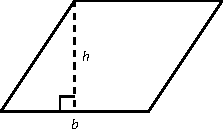
\includegraphics{figures/figcrossp_parallelogram1}\\
(a) \\[15pt]
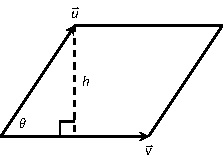
\includegraphics{figures/figcrossp_parallelogram2}\\
(b) \\
\end{tabular}
}
We illustrate using Equation \eqref{eq:crossp1} in the following example.
\index{cross product!applications!area of parallelogram}\\

\example{ex_crossp4}{Finding the area of a parallelogram}{
\begin{enumerate}
	\item Find the area of the parallelogram defined by the vectors $\vecu = \la 2,1\ra$ and $\vecv = \la 1,3\ra$.
	\item	Verify that the points $A = (1,1,1)$, $B = (2,3,2)$, $C = (4,5,3)$ and $D = (3,3,2)$ are the vertices of a parallelogram. Find the area of the parallelogram.
\end{enumerate}
}
{\begin{enumerate}
	\item Figure \ref{fig:crossp4}(a) sketches the parallelogram defined by the vectors $\vec u$ and $\vec v$. We have a slight problem in that our vectors exist in $\mathbb{R}^2$, not $\mathbb{R}^3$, and the cross product is only defined on vectors in $\mathbb{R}^3$. We skirt this issue by viewing $\vec u$ and $\vecv$ as vectors in the $x-y$ plane of $\mathbb{R}^3$, and rewrite them as $\vec u = \la 2,1,0\ra$ and $\vecv =\la 1,3,0\ra$. We can now compute the cross product. 
	It is easy to show that $\crossp uv = \la 0,0,5\ra$; therefore the area of the parallelogram is $A = \norm{\crossp uv} = 5$.
	\mtable{.65}{Sketching the parallelograms in Example \ref{ex_crossp4}.}{fig:crossp4}{%
	\begin{tabular}{c}
	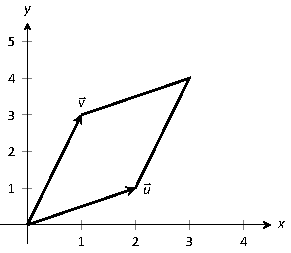
\includegraphics{figures/figcrossp4b}\\
	(a)\\[15pt]
	\myincludegraphicsthree{width=125pt,3Dmenu,activate=onclick,deactivate=onclick,
3Droll=0,
3Dortho=0.004,
3Dc2c=.42 .87 .26,
3Dcoo=61 60 63,
3Droo=250,
3Dlights=Headlamp,add3Djscript=asylabels.js}{scale=1.25,trim=4mm 5mm 4mm 5mm,clip=true}{figures/figcrossp4a}\\
	%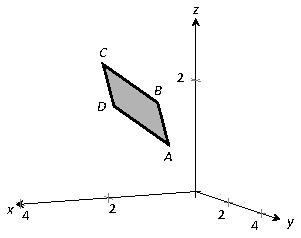
\includegraphics{figures/figcrossp4a}\\
	(b)
	\end{tabular}
	}
	\item		To show that the quadrilateral $ABCD$ is a parallelogram (shown in Figure \ref{fig:crossp4}(b)), we need to show that the opposite sides are parallel. We can quickly show that $\overrightarrow{AB} =\overrightarrow{DC} = \la 1,2,1\ra$ and $\overrightarrow{BC} = \overrightarrow{AD} = \la 2,2,1\ra$. We find the area by computing the magnitude of the cross product of $\overrightarrow{AB}$ and $\overrightarrow{BC}$:
\[
\overrightarrow{AB} \times \overrightarrow{BC} = \la 0,1,-2\ra \quad \Rightarrow \quad \norm{\overrightarrow{AB}\times\overrightarrow{BC}} = \sqrt{5} \approx 2.236.
\]
\end{enumerate}
\vskip-\baselineskip
}\\

This application is perhaps more useful in finding the area of a triangle (in short, triangles are used more often than parallelograms). We illustrate this in the following example.\\

\mfigure{.25}{Finding the area of a triangle in Example \ref{ex_crossp5}.}{fig:crossp5}{figures/figcrossp5}

\example{ex_crossp5}{Area of a triangle}{
Find the area of the triangle with vertices $A=(1,2)$, $B=(2,3)$ and $C=(3,1)$, as pictured in Figure \ref{fig:crossp5}.}
{We found the area of this triangle in Example \ref{ex_abc4} to be $1.5$ using integration. There we discussed the fact that finding the area of a triangle can be inconvenient using the ``$\frac12bh$'' formula as one has to compute the height, which generally involves finding angles, etc. Using a cross product is much more direct.

We can choose any two sides of the triangle to use to form vectors; we choose $\overrightarrow{AB} = \la 1,1\ra$ and $\overrightarrow{AC}=\la 2,-1\ra$. As in the previous example, we will rewrite these vectors with a third component of 0 so that we can apply the cross product. The area of the triangle is
\[
\frac12\norm{\overrightarrow{AB}\times\overrightarrow{AC}} = \frac12\norm{\la 1,1,0\ra \times \la 2,-1,0\ra} = \frac12\norm{\la 0,0,-3\ra} = \frac32.
\]
We arrive at the same answer as before with less work.
}\\



\pagebreak

\noindent\textbf{Volume of a Parallelepiped}

The three dimensional analogue to the parallelogram is the \textbf{parallelepiped}. Each face is parallel to the face opposite face, as illustrated in Figure \ref{fig:crossp_parallelepiped}. The volume of any three-dimensional solid whose cross-sectional area is a constant is given by $V=B\cdot h$, where $B$ is the area of the base (the constant cross-sectional area), and $h$ is the height. To determine a formula for the volume, we refer to Figure \ref{fig:parallelepiped_volume}. By crossing $\vec v$ and $\vec w$, one gets a vector whose magnitude is the area of the base, and whose direction is perpendicular to the parallelogram forming the base of the solid. We can then see that the height of the parallelepiped is equal to the length of the projection of the vector $\vec u$ onto $\crossp vw$. Thus, our volume is given by:
\begin{align*}
V & = B\cdot h\\
  & = \len{\crossp vw}\cdot \len{\operatorname{proj}_{\crossp vw}\vec{u}}\\
  & = \len{\crossp vw}\cdot\len{\left(\frac{\vec{u}\boldsymbol{\cdot}(\crossp vw)}{\len{\crossp vw}^2}\right)(\crossp vw)}\\
  & = \len{\crossp vw}\frac{\abs{\vec{u}\boldsymbol{\cdot}(\crossp vw)}}{\len{\crossp vw}^2}\len{\crossp vw}\\
  & = \abs{\vec{u}\boldsymbol{\cdot}(\crossp vw)}.
\end{align*}

\mfigurethree{width=75pt,3Dmenu,activate=onclick,deactivate=onclick,
3Droll=0,
3Dortho=0.0045,
3Dc2c=.84 .46 .26,
3Dcoo=0 110 86,
3Droo=150,
3Dlights=Headlamp,add3Djscript=asylabels.js}{}{.8}{A parallelepiped is the three dimensional analogue to the parallelogram.}{fig:crossp_parallelepiped}{figures/figcrosspparallelpiped}
%\mfigure{.53}{A parallelepiped is the three dimensional analogue to the parallelogram.}{fig:crossp_parallelepiped}{figures/figcrosspparallelpiped}
\index{cross product!applications!volume of parallelepiped}

Thus the volume of a parallelepiped defined by vectors $\vecu$, $\vecv$ and $\vec w$ is 
\begin{equation}
V = \abs{\vecu\boldsymbol{\cdot} (\crossp vw)}.\label{eq:crossp2}
\end{equation}
Note how this is the Scalar Triple Product, first seen in Theorem \ref{thm:cross_prod_prop}. Applying the identities given in the theorem shows that we can apply the Scalar Triple Product in any ``order'' we choose to find the volume. That is,
\[
V = |\vecu\boldsymbol{\cdot}(\crossp vw)| = |\vec u\boldsymbol{\cdot} (\crossp wv)| = |(\crossp uv)\boldsymbol{\cdot} \vecw|,\quad \text{etc.}
\]

\mfigure[width=0.95\marginparwidth]{.55}{Determining the volume of a parallelepiped}{fig:parallelepiped_volume}{figures/parallelepiped2}

\example{ex_crossp6}{Finding the volume of parallelepiped}{
Find the volume of the parallelepiped defined by the vectors $\vecu = \la 1,1,0\ra$, $\vecv = \la -1,1,0\ra$ and $\vecw = \la 0,1,1\ra$. 
}
{We apply Equation \eqref{eq:crossp2}. We first find $\crossp vw =\la 1,1,-1\ra$. Then
\[
|\vec u\cdot(\crossp vw)| = |\la 1,1,0\ra \cdot \la1,1,-1\ra| = 2.
\]
So the volume of the parallelepiped is 2 cubic units.
\mfigurethree{width=125pt,3Dmenu,activate=onclick,deactivate=onclick,
3Droll=0,
3Dortho=0.0045,
3Dc2c=4 4 2,
3Dcoo=0 50 50,
3Droo=150,
3Dlights=Headlamp,add3Djscript=asylabels.js}{}{.3}{A parallelepiped in Example \ref{ex_crossp6}.}{fig:crossp6}{figures/figcrossp6}
%\mfigure{.3}{A parallelepiped in Example \ref{ex_crossp6}.}{fig:crossp6}{figures/figcrossp6}
}\\

Let's take another look at how Equation \eqref{eq:crossp2} is computed in terms of our formulas for the dot and cross products. With $\vec u = \la u_1, u_2, u_3\ra, \vec v = \la v_1, v_2, v_3\ra$, and $\vec w = \la w_1, w_2, w_3\ra$, we have
\begin{align*}
\vec{u}\boldsymbol{\cdot}(\crossp vw) & = \la u_1, u_2, u_3\ra \boldsymbol{\cdot}\left\langle \bvm v_2 & v_3\\w_2&w_3\evm, -\bvm v_1 & v_3\\ w_1 & w_3\evm, \bvm v_1 & v_2\\ w_1 & w_2\evm\right\rangle\\
 & = u_1\bvm v_2 & v_3\\w_2&w_3\evm - u_2\bvm v_1 & v_3\\ w_1 & w_3\evm + u_3\bvm v_1 & v_2\\ w_1 & w_2\evm.
\end{align*}
Compare this with our determinant formula for computing the cross product,
\[
\crossp vw = \bvm \veci & \vecj & \veck\\ v_1 & v_2 & v_3\\ w_1 & w_2 & w_3\evm = \bvm v_2 & v_3\\w_2&w_3\evm\veci - \bvm v_1 & v_3\\ w_1 & w_3\evm\vecj + \bvm v_1 & v_2\\ w_1 & w_2\evm\veck.
\]
If we replace the unit vectors $\veci, \vecj, veck$ in the above equation with the components of $\vec{u}$, we arrive at our first instance of a \textbf{$3\times 3$ determinant}, along with a method for computing such an object:
\[
\bvm u_1 & u_2 & u_3\\ v_1 & v_2 & v_3\\ w_1 & w_2 & w_3\evm = u_1 \bvm v_2 & v_3\\ w_2 & w_3\evm - u_2\bvm v_1 & v_3\\ w_1 & w_3\evm + u_3\bvm v_1 & v_2\\ w_1 & w_2\evm = \vec u\boldsymbol{\cdot}(\crossp vw).
\]
We will return to our study of determinants in Section \ref{sec:determinant_1}, where we will learn techniques for efficiently computing determinants of any size.

While this application of the Scalar Triple Product is interesting, it is not used all that often: parallelepipeds are not a common shape in physics and engineering. (It is, however, essential to understanding the change of variables formula for multiple integrals in Calculus.) The last application of the cross product is very applicable in engineering.\\

\noindent\textbf{Torque}\\

\textbf{Torque} is a measure of the turning force applied to an object. A classic scenario involving torque is the application of a wrench to a bolt. When a force is applied to the wrench, the bolt turns. When we represent the force and wrench with vectors $\vec F$ and $\vec \ell$, we see that the bolt moves (because of the threads) in a  direction orthogonal to $\vec F$ and $\vec \ell$. Torque is usually represented by the Greek letter $\tau$, or tau, and has units of N$\cdot$m, a Newton--meter, or ft$\cdot$lb, a foot--pound.\index{cross product!applications!torque}

While a full understanding of torque is beyond the purposes of this book, when a force $\vec F$ is applied to a lever arm $\vec \ell$, the resulting torque is \begin{equation}\vec \tau = \crossp \ell F.\label{eq:crossp3}\end{equation}

\example{ex_crossp7}{Computing torque}{
A lever of length 2ft makes an angle with the horizontal of $45^\circ$. Find the resulting torque when a force of 10lb is applied to the end of the level where:
\begin{enumerate}
	\item the force is perpendicular to the lever, and
	\item	the force makes an angle of $60^\circ$ with the lever, as shown in Figure \ref{fig:crossp7}.
\end{enumerate}
}
{\begin{enumerate}
	\item We start by determining vectors for the force and lever arm. Since the lever arm makes a $45^\circ$ angle with the horizontal and is 2ft long, we can state that $\vec \ell = 2\la \cos 45^\circ,\sin 45^\circ\ra = \la \sqrt2,\sqrt2\ra.$
	
	Since the force vector is perpendicular to the lever arm (as seen in the left hand side of Figure \ref{fig:crossp7}), we can conclude it is making an angle of $-45^\circ$ with the horizontal. As it has a magnitude of 10lb, we can state $\vec F = 10\la \cos (-45^\circ), \sin(-45^\circ)\ra = \la 5\sqrt2,-5\sqrt2\ra.$
	
	Using Equation \eqref{eq:crossp3} to find the torque requires a cross product. We again let the third component of each vector be 0  and compute the cross product:
	\begin{align*}
	\vec\tau &= \crossp \ell F \\
				&= \la \sqrt2,\sqrt2,0\ra \times \la 5\sqrt2,-5\sqrt2,0\ra \\
				&= \la 0,0,-20\ra
	\end{align*}
	This clearly has a magnitude of 20 ft-lb.
	
	We can view the force and lever arm vectors as lying ``on the page''; our computation of $\vec\tau$ shows that the torque goes ``into the page.'' This follows the Right Hand Rule of the cross product, and it also matches well with the example of the wrench turning the bolt. Turning a bolt clockwise moves it in.
	
	\item		Our lever arm can still be represented by $\vec \ell = \la \sqrt2,\sqrt2\ra$. As our force vector makes a $60^\circ$ angle with $\vec \ell$, we can see (referencing the right hand side of the figure) that $\vec F$ makes a $-15^\circ$ angle with the horizontal. Thus 
	\begin{align*}
	\vec F = 10\la \cos-15^\circ,\sin-15^\circ\ra &= \la \frac{5(1+\sqrt3)}{\sqrt2},-\frac{5(1+\sqrt3)}{\sqrt2}\ra \\
	&\approx \la 9.659,-2.588\ra.\end{align*}
	
	We again make the third component 0 and take the cross product to find the torque:
	\begin{align*}
	\vec\tau &= \crossp \ell F\\
					&= \la \sqrt2,\sqrt2,0\ra \times  \la \frac{5(1+\sqrt3)}{\sqrt2},-\frac{5(1+\sqrt3)}{\sqrt2},0\ra\\
					&= \la 0,0,-10\sqrt3\ra\\
					&\approx \la 0,0,-17.321\ra.
	\end{align*}
	As one might expect, when the force and lever arm vectors \textit{are} orthogonal, the magnitude of force is greater than when the vectors \textit{are not} orthogonal.
\end{enumerate}
\vskip-\baselineskip
}\\

\mfigure{.6}{Showing a force being applied to a lever in Example \ref{ex_crossp7}.}{fig:crossp7}{figures/figcrossp7}

While the cross product has a variety of applications (as noted in this chapter), its fundamental use is finding a vector perpendicular to two others. Knowing a vector is orthogonal to two others is of incredible importance, as it allows us to find the equations of lines and planes in a variety of contexts. The importance of the cross product, in some sense, relies on the importance of lines and planes, which see widespread use throughout engineering, physics and mathematics. We study lines and planes in the next two sections. 

\printexercises{exercises/10_04_exercises}

